%%%%%%%%%%%%%%%%%%%%%%%%%%%%%%%%%%%%%%%%%%%%%%%%%%%%%%%%%%%%%%%%%%%%%%%%%%
% Normalized voltage u_2(alpha)/u_2(alpha=0)
%%%%%%%%%%%%%%%%%%%%%%%%%%%%%%%%%%%%%%%%%%%%%%%%%%%%%%%%%%%%%%%%%%%%%%%%%%
\begin{solutionfigure}[htb]

    %   \documentclass{standalone}
    %   \usepackage{pgfplots}
    %   \pgfplotsset{compat=1.18} % Kompatibilität für neuere Versionen
           \centering
           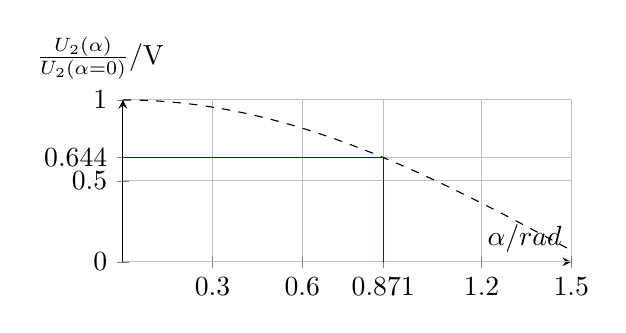
\begin{tikzpicture}
               \begin{axis}[
                   % x/y range adjustment
                   xmin=0, xmax=85.94,
                   ymin=0, ymax=1,
                   samples=500,
                   axis y line=center,
                   axis x line=center,
                   extra y ticks=0,
                   % Label text
                   xlabel={$\alpha / \text{rad}$},
                   ylabel={$\frac{ U_\mathrm{2}(\alpha)}{U_\mathrm{2}(\alpha=0)} /\mathrm{V}$},
                   % Label adjustment
                  % x label style={at={(axis description cs:1,0.5)},anchor=west},
                   y label style={at={(axis description cs:-.05,.97)},anchor=south,yshift=0.2cm},
                   width=0.6\textwidth,
                   height=0.3\textwidth,
                   % x-Ticks
                   xtick={0,17.19,34.38,49.9,68.76,85.94},
                   xticklabels={0,0.3,0.6,0.871,1.2,1.5},
                   xticklabel style = {anchor=north},
                   % y-Ticks
                   ytick={0,0.5,0.644,1},
                   yticklabels={0,0.5,0.644,1},
                   yticklabel style = {anchor=east},
                   % Grid layout
                   grid,
                   %grid style={line width=.1pt, draw=gray!10},
                   %major grid style={line width=.2pt,draw=gray!90},
               ]
               % Voltage u_2(alpha)/u_2(alpha=0)
               \addplot[black, domain= 0:85.94,dashed] {cos(x)}; 
               % u_2(alpha)/u_2(alpha=0) when alpha = 0.87               
               \addplot[color=blue,solid] coordinates{
                (49.9,0)
                (49.9, 0.644)
            };
            \addplot[color=blue,solid] coordinates{
                (0,0.644)
                (49.9, 0.644)
            };
                       
           \end{axis}     
           \end{tikzpicture}
           \caption{normalized curve for $\frac{ U_\mathrm{2}(\alpha)}{U_\mathrm{2}(\alpha=0)}$ with $\alpha = 0.871$.}
           \label{sfig:ex06_output_voltage_6_1_2}
   \end{solutionfigure}